\documentclass{VUMIFPSkursinis}
\usepackage{algorithmicx}
\usepackage{algorithm}
\usepackage{algpseudocode}
\usepackage{amsfonts}
\usepackage{amsmath}
\usepackage{array}
\usepackage{bm}
\usepackage{caption}
\usepackage{color}
\usepackage{float}
\usepackage{graphicx}
\usepackage{listings}
\usepackage{longtable}
\usepackage{subfig}
\usepackage{wrapfig}
\usepackage{enumitem}

\usepackage{csvsimple}

\usepackage[tableposition=top]{caption}
%PAKEISTA, tarpai tarp sąrašo elementų
\setitemize{noitemsep,topsep=0pt,parsep=0pt,partopsep=0pt}
\setenumerate{noitemsep,topsep=0pt,parsep=0pt,partopsep=0pt}

\newcolumntype{L}[1]{>{\raggedright\let\newline\\\arraybackslash\hspace{0pt}}m{#1}}
\newcolumntype{C}[1]{>{\centering\let\newline\\\arraybackslash\hspace{0pt}}m{#1}}
\newcolumntype{R}[1]{>{\raggedleft\let\newline\\\arraybackslash\hspace{0pt}}m{#1}}

% Titulinio aprašas
\university{Vilniaus universitetas}
\faculty{Matematikos ir informatikos fakultetas}
\department{Programų sistemų katedra}
\title{Kompiuterinių žaidimų projektavimas ir kūrimas. „Out of Bounds“ projekto ir dizaino dokumentacija}
\titleineng{Video Game design and development. „Out of Bounds“ project and design documentation}
\papertype{Trečioji užduotis}
\supervisor{Asist. Dr. Žilvinas Ledas}

\date{Vilnius – \the\year}

% Nustatymai
% \setmainfont{Palemonas}   % Pakeisti teksto šriftą į Palemonas (turi būti įdiegtas sistemoje)
\bibliography{bibliografija}

\begin{document}
	
% PAKEISTA	
\maketitle

%TURINYS
\tableofcontents



% -----------------------------------------------------------------
% ------------------------- 1. APŽVALGA ---------------------------
% -----------------------------------------------------------------
\section{Apžvalga}


% -------------------------------------------
% --------- 1.1 Idėjos aprašymas ------------
% -------------------------------------------
\subsection{Idėjos aprašymas}
\textit{Out of Bounds} - žaidimas, kuriame valdant veikėjus turinčius unikalių super galių, kovojama dėl išlikimo sumo idėja paremtoje arenoje. Žaidėjai stengiasi išstumti vienas kitą iš arenos, pasitelkdami žalos darymo sistemą, kuri suteikia galimybę žaidėją padaryti lengvesniu ir taip gerokai palengvinti išstūmimą iš arenos. Laimi paskutinis išlikęs arenoje žaidėjas. P.S. yra ginklų.


% -------------------------------------------
% -------- 1.2 Bendra informacija -----------
% -------------------------------------------
\subsection{Bendra informacija}
\begin{itemize}
    \item \textbf{Kalba} - anglų.
    \item \textbf{Žanras} - veiksmo, muštynių.
    \item \textbf{Žaidėjų skaičius} - nuo 2 iki 4 (nėra galimybės kovoti prieš kompiuterio valdomus veikėjus).
    \item \textbf{Platforma} - Windows 10.
    \item \textbf{Valdymo įrenginiai} - klaviatūra ir pelė arba Xbox One™ pultelis.
    \item \textbf{Grafikos stilius} - minimalistinis, futuristinis, pabrėžiamos paprasčiausios formos (apskritimas, trikampis, kvadratas) bei akcentuojama balta spalva.
    \item \textbf{Muzikos stilius} - elektroninė, futuristinio skambesio, greitesnio tempo muzika.
\end{itemize}


% -----------------------------------------------------------------
% --------------------------- 2. EIGA -----------------------------
% -----------------------------------------------------------------
\section{Eiga}
Tolesniuose poskyriuose pristatomi detalūs žaidimo eigos elementai.


% -------------------------------------------
% -------------- 2.1 Tikslas ----------------
% -------------------------------------------
\subsection{Tikslas}
\textit{Out of Bounds} žaidimo tikslas - likti paskutiniam gyvam žaidėjui arenoje. Mirštama patekus už areną ribojančio apskritimo ribų 2 sekundėms.


% -------------------------------------------
% -------- 2.2 Žaidimo eigos struktūra ------
% -------------------------------------------
\subsection{Žaidimo eigos struktūra}
% Idėja kaip pakeisti 2.1 pirmąją pastraipą
Pagrindiniame meniu paspaudžiama "Pradėti žaidimą". Naujai atsidariusiame lange žaidėjai išsirenka veikėjus, kuriuos valdys. Juos patvirtinus parodomas arenos pasirinkimo langas, kuriame žaidėjai taip pat sutaria iki kiek pergalių bus kovojama pasirinktoje arenoje. Įtvirtinus pasirinkimus pradedamas žaidimas.

Prasidėjus naujam raundui veikėjai atsiranda nustatytose arenos vietose ir atbuliniam skaičiavimui nuo 3 pasiekus 0 pradedama kovoti. Žaidėjai kovoja tol, kol lieka vienintelis gyvas veikėjas arenoje, kuris tampa raundo nugalėtoju. Tuomet prasideda naujas raundas. Žaidėjas, laimėjęs nurodytą raundų kiekį tampa žaidimo nugalėtoju.


% -------------------------------------------
% ----------- 2.3 Kovos elementai -----------
% -------------------------------------------
\subsection{Kovos elementai}
Kiekvienas veikėjas kovą pradeda su 0\% žalos ir patyrus žalą šis procentas didėja, tačiau negali viršyti 500\% (žalos lubos). Žalą daro priešininkų ginklai, galios ir gebėjimai. Patiriant žalą veikėjas yra nustumiamas kryptimi, sutampančia su žalos vektoriaus kryptimi. Žalos ir pastūmimo kiekis priklauso nuo konkretaus ginklo, galios ar gebėjimo. Pastūmimo kiekis yra dauginamas iš veikėjo žalos kiekio (kuo daugiau žalos, tuo jis bus toliau pastumiamas).

% -------------------------------
% ------- 2.4 Gebėjimai ---------
% -------------------------------

\subsection{Gebėjimai}
Visi žaidimo veikėjai pasižymi vienodais gebėjimais:
\begin{itemize}
    \item \textbf{Run} (\textit{bėgti}) - judėti į kairę arba dešinę.
    \item \textbf{Dash} (\textit{veržtis}) - leidžia trumpam intervalui tapti nesužeidžiamu ir staigiai pajudėti apibrėžtą atstumą kryptimi į kurią taikomasi.
    \item \textbf{Punch} (\textit{trenkti}) - smūgiuoti, darant labai mažai žalos ir mažai pastumiant priešininką.
    \item \textbf{Shoot} (\textit{šauti}) - iššauti iš laikomo ginklo.
    \item \textbf{Jump} (\textit{pašokti}) - pašokti į viršų.
    \item \textbf{Double jump} (\textit{antrasis pašokimas}) - esant ore dar kartą pašokti aukštyn.
    \item \textbf{Crouch} (\textit{pritūpti}) - pritūpti.
    \item \textbf{Aim} (\textit{taikytis}) - veikėjas gali atskirai taikytis naudojant pultelio dešiniąją svirtelę arba pelę (jeigu pultelio dešinioji svirtelė yra neutralioje pozicijoje, tada veikėjas taikosi ten, kur nulenkta kairioji svirtelė).
    \item \textbf{Shield} (\textit{gintis}) - trumpalaikis gynimasis 1 sekundės trukmės. Naudoti galima kas 3 sekundes. Apgina veikėją nuo visų atakų iš tos krypties į kurią tuo metu jis taikosi    .
\end{itemize}


% -------------------------------------------
% -------------- 2.5 Veikėjai ---------------
% -------------------------------------------
\subsection{Veikėjai}
Visi veikėjai turi bendrus gebėjimus ir po 2 unikalias galias. Unikalios galios turi atvėsimo trukmes (angl. cooldown) priklausančias nuo pačios galios.


% -------------------------------
% -------- 2.5.1 Malean ---------
% -------------------------------
\subsubsection{Malean}
Malean buvo specialiai sukurtas kovoms arenose. Jis neturi jausmų, emocijų ir jo vienintelis tikslas yra laimėti. Kiekvieną kartą jam pralaimėjus yra perkraunama atmintis, kad jis nebūtų paveiktas to liūdno prisiminimo.

Malean galios:
\begin{itemize}
    \item \textbf{Juodoji skylė} - iššauna juodąją skylę, kuri materializuojasi nuskridusi tam tikrą atstumą ir traukia priešus į save 2 sekundes. Postūmio stiprumas didėja kuo arčiau veikėjas yra juodosios skylės. Jei veikėjas įtraukiamas į juodąją skylę patiria žalą.
    \begin{itemize}
        \item \textbf{Žala} - vidutinė
        \item \textbf{Postūmis} - nuo mažo iki vidutinio
        \item \textbf{Atvėsimas} - ilgas
    \end{itemize}
    \item \textbf{Kiborgo smūgis} - su trumpu užsimojimu trenkia į žemę arba į stogą (galima paleisti tik esant ore, paleidimo kryptis (viršų arba apačią) priklauso nuo veikėjo greičio krypties) ir priešininkai stovintys tam tikru atstumu ant trenktos platformos patiria vidutinį postūmį ir mažai žalos.
    \begin{itemize}
        \item \textbf{Žala} - maža
        \item \textbf{Postūmis} - vidutinis
        \item \textbf{Atvėsimas} - vidutinis
    \end{itemize}
\end{itemize}

\begin{figure}[H]
    \centering
    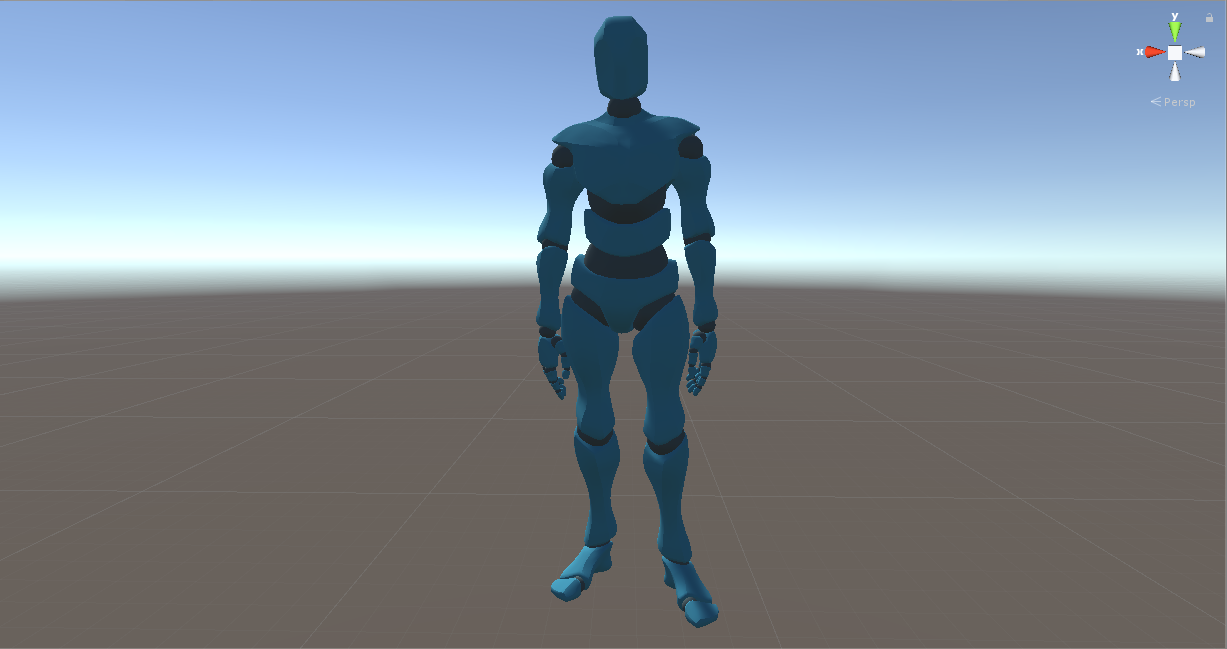
\includegraphics[scale=0.3]{img/Characters/Malean.png}
    \caption{Pavyzdinis Malean modelis}
    \label{img:malean}
\end{figure}

% -------------------------------
% ------- 2.5.2 Valkyrie --------
% -------------------------------
\subsubsection{Valkyrie}
Iš ShanShan-52 planetos, Valkyrie nėra sutikusi varžovo, kurio negalėtų nugalėti. Mamos sukonstruotas mechaninis kostiumas, iššaunantis priešus sekiojančias raketas bei gebėjimas tapti nematomai trumpam periodui suteikė jai vietą savo gimtosios planetos specialių pajėgų padalinyje. 

Valkyrie galios:
\begin{itemize}
    \item \textbf{Nematomumas} - 2 sekundėms veikėjas tampa nematomas ir šiek tiek pasigydo;
    \begin{itemize}
        \item \textbf{Žala} - jokios
        \item \textbf{Postūmis} - jokio
        \item \textbf{Atvėsimas} - trumpas
        \item \textbf{Gydymasis} - silpnas
    \end{itemize}
    \item \textbf{Persekiojančios raketos} - iššauna raketas, kurios persekioja varžovus.
    \begin{itemize}
        \item \textbf{Žala} - vidutinė
        \item \textbf{Postūmis} - vidutinis
        \item \textbf{Atvėsimas} - ilgas
    \end{itemize}
\end{itemize}

\begin{figure}[H]
    \centering
    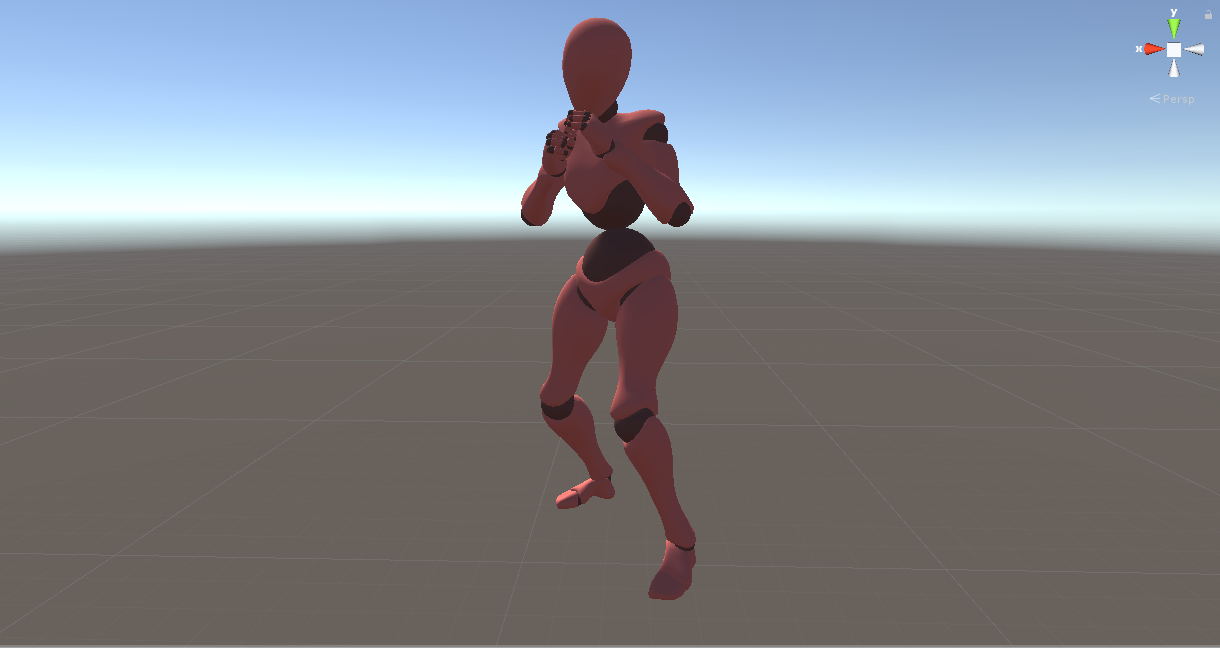
\includegraphics[scale=0.3]{img/Characters/Valkyrie.png}
    \caption{Pavyzdinis Valkyrie modelis}
    \label{img:valkyrie}
\end{figure}

% -------------------------------
% ----- 2.5.3 Penkratjevas ------
% -------------------------------
\subsubsection{Penkratjevas}
Jis yra piktas ir įniršęs, nes neranda darbo. Dėl to jis pašventė savo gyvenimą atkeršyti visiems darbdaviams. Tam jis dėvi specialų apsiaustą, kuris suteikia antžmogio galių, nes jis yra teisingumo kosmonautas, prieblandos ambasadorius ir priešininkų nelaimė. 

Penkratjev galios:
\begin{itemize}
    \item \textbf{Apsikeitimas} - apsikeičia vietomis su artimiausiu kitu veikėju, kuris nutolęs iki tam tikro atstumo (jei priešas yra pakankamai toli, tada susikeisti negalima). Greičio vektoriais nesusikeičiama.
    \begin{itemize}
        \item \textbf{Žala} - nėra
        \item \textbf{Postūmis} - nėra
        \item \textbf{Atvėsimas} - vidutinis
    \end{itemize}
    \item \textbf{Pagiežos lazeris} - žaidėjas paleidžia lazerį šviesos greičiu ten, kur yra nusitaikęs. Lazeris daro žalą ir stumia priešininką, tačiau taip pat šiek tiek pastumia save priešinga lazerio iššovimo kryptimi.
    \begin{itemize}
        \item \textbf{Žala} - didelė
        \item \textbf{Postūmis} - didelis
        \item \textbf{Atvėsimas} - vidutinis
    \end{itemize}
\end{itemize}

\begin{figure}[H]
    \centering
    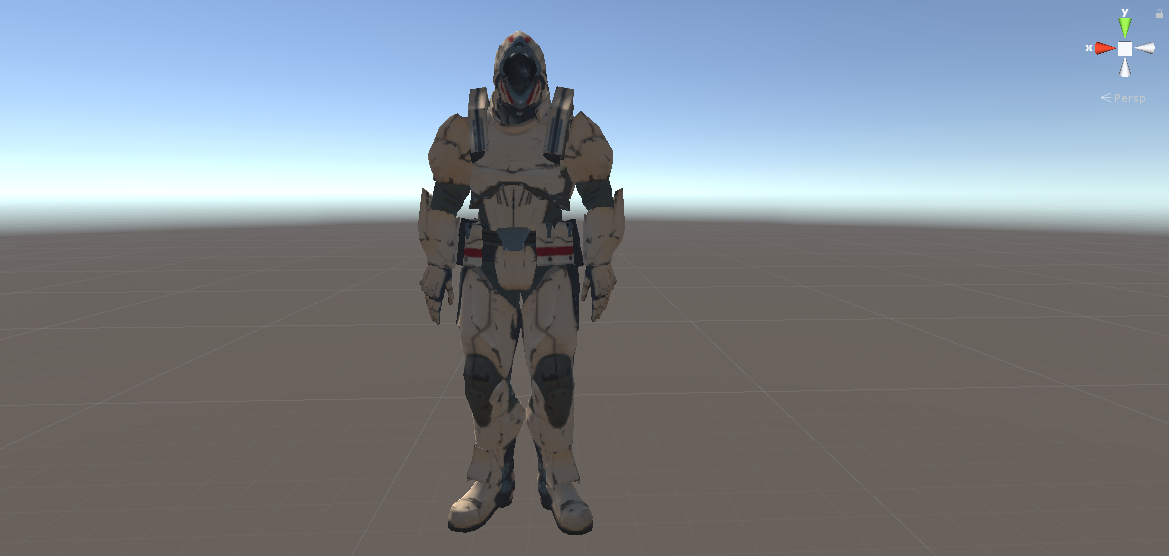
\includegraphics[scale=0.3]{img/Characters/Penkratjevas.png}
    \caption{Pavyzdinis Penkratjev modelis}
    \label{img:penkratjevas}
\end{figure}

% -------------------------------
% -------- 2.5.4 Bonbon ---------
% -------------------------------
\subsubsection{Bonbon}
Vieni sako, kad jis negali pralaimėti, nes jis mirė jau seniai, kiti sako kad jis buvęs piratas. Viskas ką mes žinome yra tai, kad jo vardas Bonbon. 

Bonbon galios:
\begin{itemize}
    \item \textbf{Kaupiamas smūgis} - smūgis kuriam kaupti reikia laiko (galima judėti kaupiant), nustūmimo galia priklauso nuo laiko kurį ši ataka buvo kaupiama;
    \begin{itemize}
        \item \textbf{Žala} - nuo mažos iki vidutinės
        \item \textbf{Postūmis} - nuo mažo iki didelio
        \item \textbf{Atvėsimas} - trumpas
    \end{itemize}
    \item \textbf{Akmens forma} - sustingsta, tuo metu veikėjas juda lėčiau ir toliau gauna žalą, bet jo neįmanoma nustumti.
    \begin{itemize}
        \item \textbf{Žala} - jokios
        \item \textbf{Postūmis} - jokio
        \item \textbf{Atvėsimas} - ilgas
    \end{itemize}
\end{itemize}

\begin{figure}[H]
    \centering
    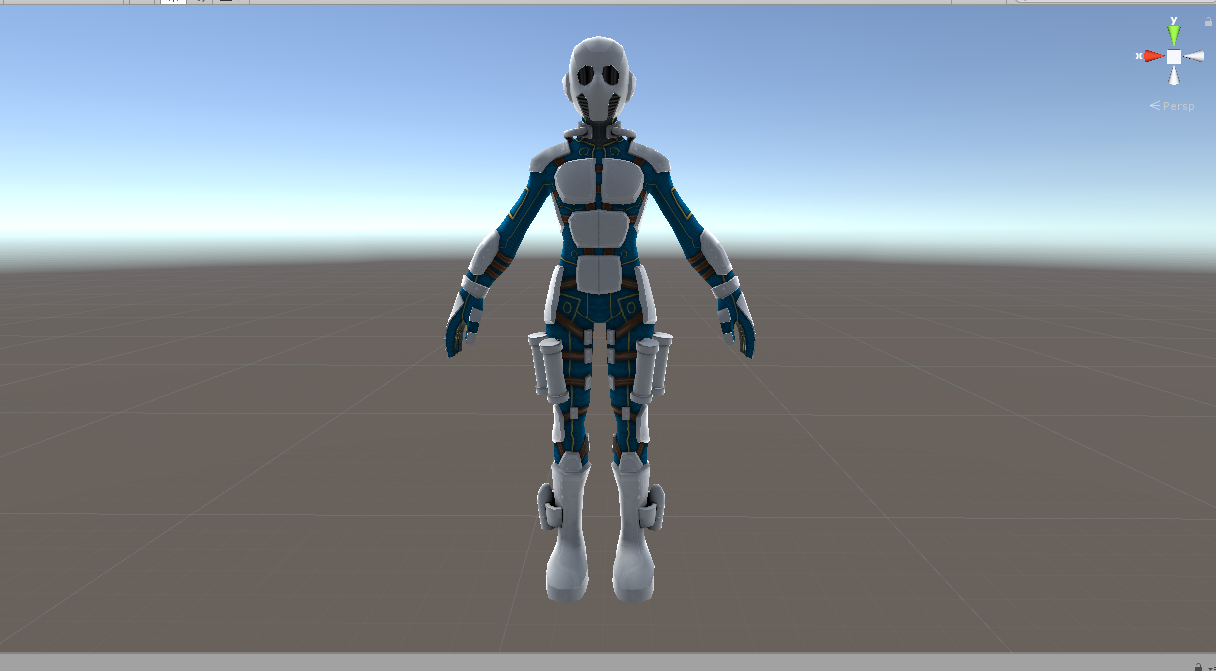
\includegraphics[scale=0.3]{img/Characters/Bonbon.png}
    \caption{Pavyzdinis Bonbon modelis}
    \label{img:bonbon}
\end{figure}



% -------------------------------------------
% -------------- 2.6 Ginklai ----------------
% -------------------------------------------
\subsection{Ginklai}
Kiekvienas veikėjas pradeda žaidimą turėdamas pistoletą. Pistoletas turi begalinį kiekį šovinių, tačiau jis yra pats silpniausias ginklas. Kiti ginklai nustatytu intervalu nukrenta iš ekrano viršaus į areną ir veikėjas, jei turi tik pistoletą, užlipęs ant jo jį pasiima. Kai veikėjas turi pasiėmęs ginklą, jis šaudo tik iš to ginklo (iš pistoleto šaudyti negali). Paimami ginklai turi ribotą šovinių kiekį ir šiems pasibaigus paimtas ginklas pradingsta ir veikėjas toliau gali šaudyti iš pistoleto.


% -------------------------------
% ------ 2.6.1 Pistoletas -------
% -------------------------------
\subsubsection{Pistoletas}
Tai yra pats silpniausias ginklas.

Pistoleto savybės:
\begin{itemize}
    \item \textbf{Šaudymo greitis} - mažas;
    \item \textbf{Žala} - maža;
    \item \textbf{Postūmis} - mažas;
    \item \textbf{Maksimalus panaudojimų skaičius} - begalinis.
\end{itemize}

\begin{figure}[H]
    \centering
    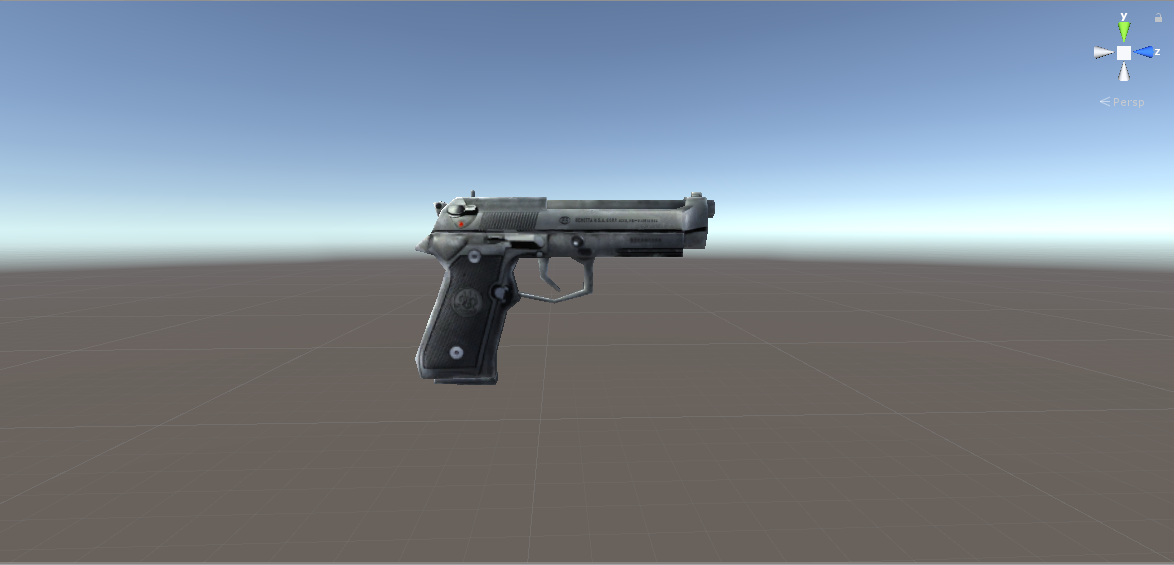
\includegraphics[scale=0.3]{img/Weapons/Pistol.png}
    \caption{Pavyzdinis pistoleto modelis}
    \label{img:pistol}
\end{figure}

% -------------------------------
% ------ 2.6.2 Automatas --------
% -------------------------------
\subsubsection{Automatas}
Tai vienas iš ginklų, kuris atsitiktinai atsiras žemėlapiuose veikėjams naudoti kovos metu. Automato savybės:
\begin{itemize}
    \item \textbf{Šaudymo greitis} - didelis;
    \item \textbf{Žala} - maža;
    \item \textbf{Postūmis} - mažas;
    \item \textbf{Maksimalus panaudojimų skaičius} - 5.
\end{itemize}

\begin{figure}[H]
    \centering
    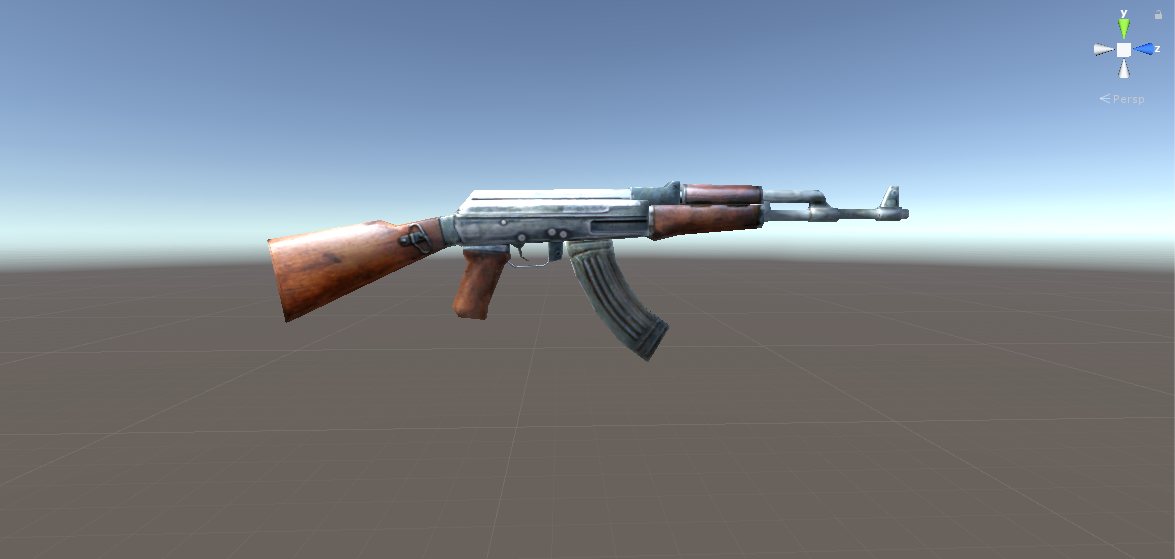
\includegraphics[scale=0.3]{img/Weapons/Rifle.png}
    \caption{Pavyzdinis automato modelis}
    \label{img:rifle}
\end{figure}

% -------------------------------
% ------ 2.6.3 Šratinis --------
% -------------------------------
\subsubsection{Šratinis}
Tai vienas iš ginklų, kuris atsitiktinai atsiras žemėlapiuose veikėjams naudoti kovos metu. Šratinio savybės:
\begin{itemize}
    \item \textbf{Šaudymo greitis} - labai mažas;
    \item \textbf{Žala} - vidutinė;
    \item \textbf{Postūmis} - vidutinis;
    \item \textbf{Maksimalus panaudojimų skaičius} - 3;
    \item \textbf{Papildoma informacija} - iššauna 4 kulkas vienu metu.
\end{itemize}

\begin{figure}[H]
    \centering
    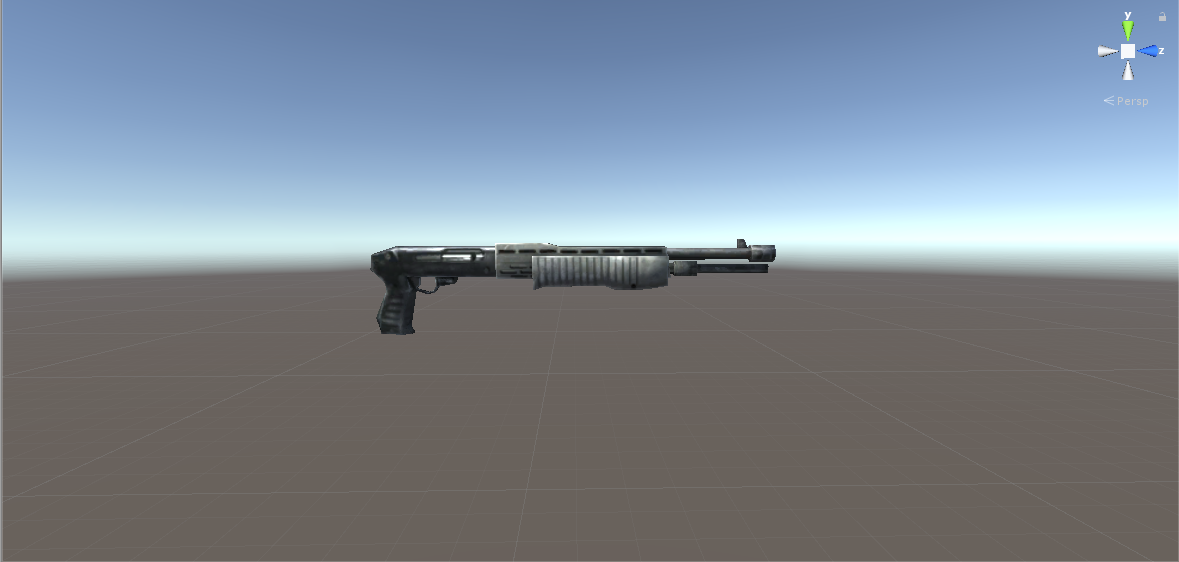
\includegraphics[scale=0.3]{img/Weapons/Shotgun.png}
    \caption{Pavyzdinis šratinio modelis}
    \label{img:shotgun}
\end{figure}

% -------------------------------
% ------ 2.6.4 Snaiperis --------
% -------------------------------
\subsubsection{Snaiperis}
Tai vienas iš ginklų, kuris atsitiktinai atsiras žemėlapiuose veikėjams naudoti kovos metu. Snaiperio savybės:
\begin{itemize}
    \item \textbf{Šaudymo greitis} - labai mažas;
    \item \textbf{Žala} - didelė;
    \item \textbf{Postūmis} - vidutinis;
    \item \textbf{Maksimalus panaudojimų skaičius} - 3.
\end{itemize}

\begin{figure}[H]
    \centering
    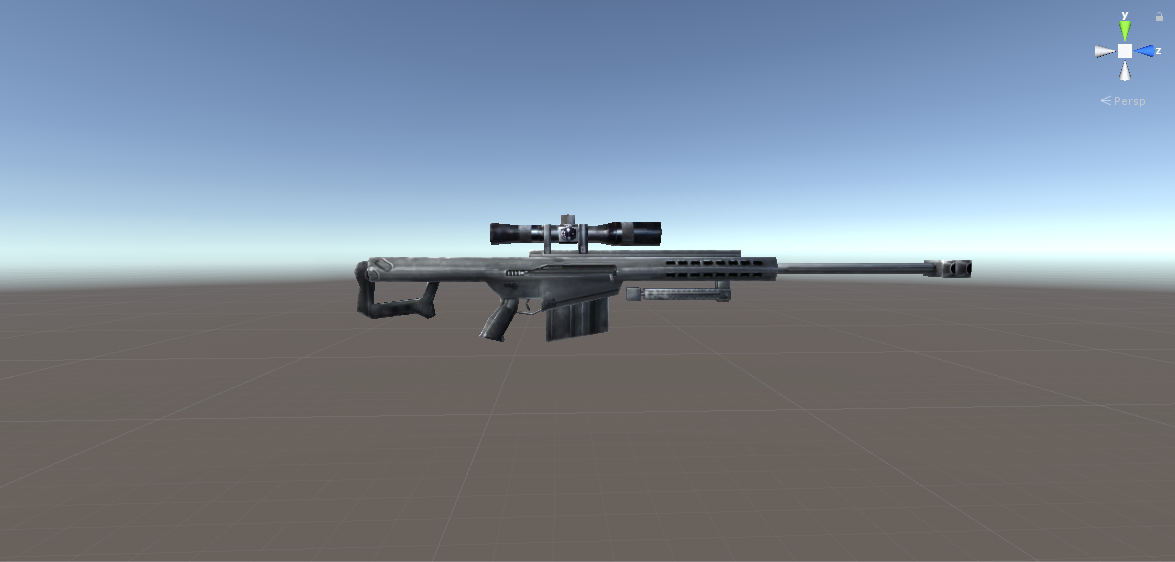
\includegraphics[scale=0.3]{img/Weapons/Sniper.png}
    \caption{Pavyzdinis snaiperio modelis}
    \label{img:sniper}
\end{figure}

% -------------------------------
% ----- 2.6.5 Raketsvaidis ------
% -------------------------------
\subsubsection{Raketsvaidis}
Tai vienas iš ginklų, kuris atsitiktinai atsiras žemėlapiuose veikėjams naudoti kovos metu. Raketsvaidžio savybės:
\begin{itemize}
    \item \textbf{Šaudymo greitis} - labai mažas;
    \item \textbf{Žala} - labai didelė;
    \item \textbf{Postūmis} - didelis;
    \item \textbf{Maksimalus panaudojimų skaičius} - 2;
    \item \textbf{Papildoma informacija} - šaudo raketomis, kurios skrenda daug lėčiau nei kulkos ir atsitrenkusios į paviršių sprogsta (žala ir postūmis sprogstant paveikia nedideliu atstumu esančius veikėjus).
\end{itemize}

\begin{figure}[H]
    \centering
    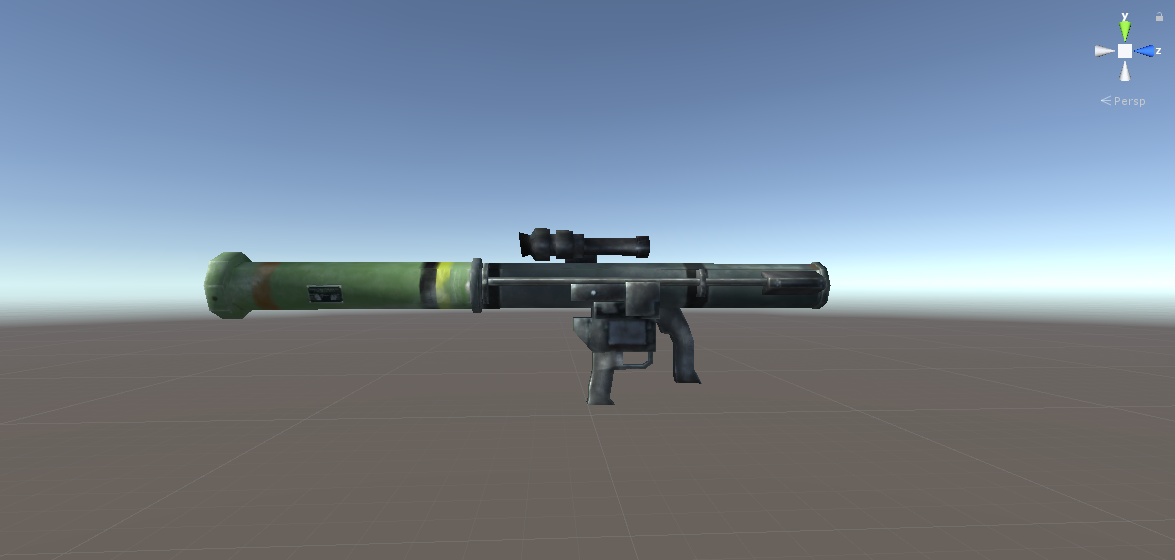
\includegraphics[scale=0.3]{img/Weapons/Rocket_launcher.png}
    \caption{Pavyzdinis raketsvaidžio modelis}
    \label{img:rocketlauncher}
\end{figure}

% -------------------------------
% ---- 2.6.6 Beisbolo lazda -----
% -------------------------------
\subsubsection{Beisbolo lazda}
Tai vienas iš ginklų, kuris atsitiktinai atsiras žemėlapiuose veikėjams naudoti kovos metu. Beisbolo lazdos savybės:
\begin{itemize}
    \item \textbf{smūgiavimo greitis} - mažas;
    \item \textbf{Žala} - vidutinė;
    \item \textbf{Postūmis} - didelis;
    \item \textbf{Maksimalus panaudojimų skaičius} - 3.
\end{itemize}

\begin{figure}[H]
    \centering
    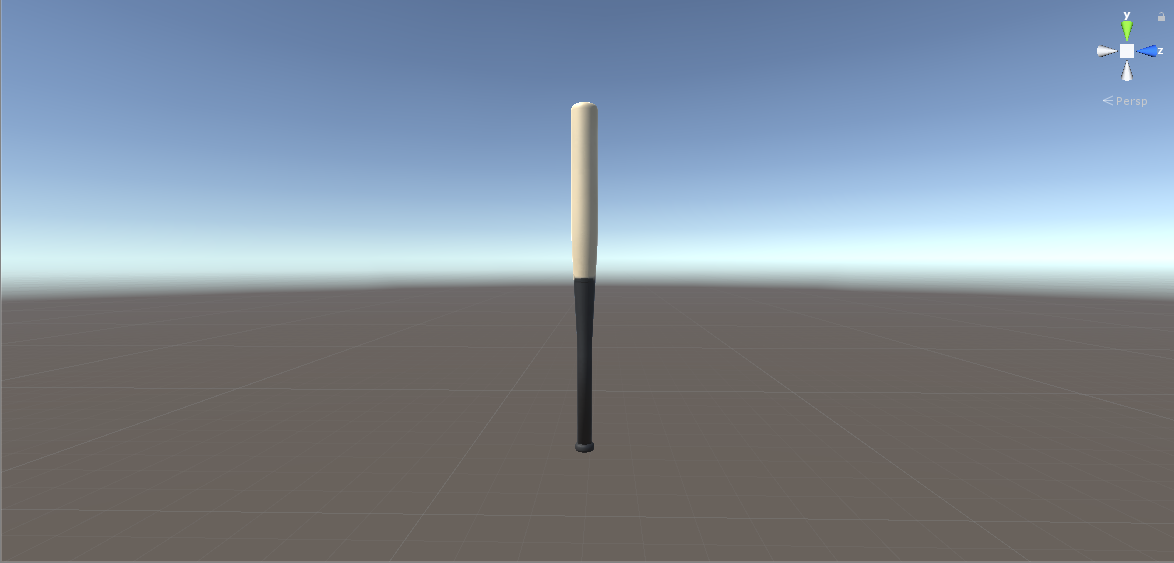
\includegraphics[scale=0.3]{img/Weapons/Baseball_bat.png}
    \caption{Pavyzdinis beisbolo lazdos modelis}
    \label{img:baseballbat}
\end{figure}

% -------------------------------
% --------- 2.6.7 Dalgis --------
% -------------------------------
\subsubsection{Dalgis}
Tai vienas iš ginklų, kuris atsitiktinai atsiras žemėlapiuose veikėjams naudoti kovos metu. Dalgio savybės:
\begin{itemize}
    \item \textbf{smūgiavimo greitis} - mažas;
    \item \textbf{Žala} - didelė;
    \item \textbf{Postūmis} - mažas;
    \item \textbf{Maksimalus panaudojimų skaičius} - 3.
\end{itemize}

\begin{figure}[H]
    \centering
    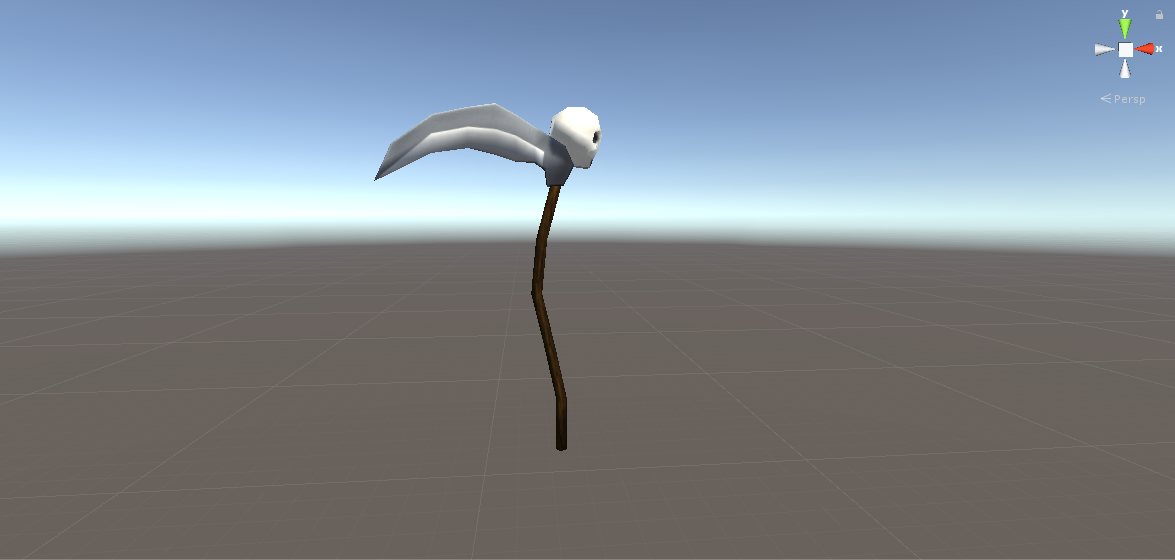
\includegraphics[scale=0.3]{img/Weapons/Scythe.png}
    \caption{Pavyzdinis dalgio modelis}
    \label{img:scythe}
\end{figure}

% -------------------------------
% --------- 2.6.8 Peilis --------
% -------------------------------
\subsubsection{Peilis}
Tai vienas iš ginklų, kuris atsitiktinai atsiras žemėlapiuose veikėjams naudoti kovos metu. Peilio savybės:
\begin{itemize}
    \item \textbf{smūgiavimo greitis} - labai didelis;
    \item \textbf{Žala} - maža;
    \item \textbf{Postūmis} - mažas;
    \item \textbf{Maksimalus panaudojimų skaičius} - 12.
\end{itemize}

\begin{figure}[H]
    \centering
    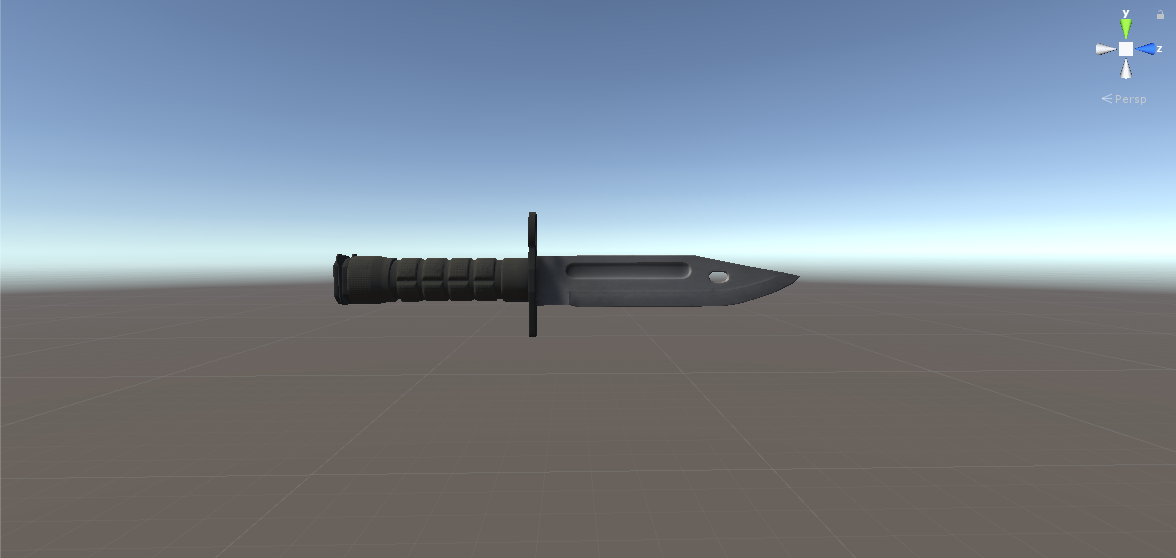
\includegraphics[scale=0.3]{img/Weapons/Knife.png}
    \caption{Pavyzdinis peilio modelis}
    \label{img:knife}
\end{figure}



% -------------------------------------------
% --------------- 2.7 Arenos ----------------
% -------------------------------------------
\subsection{Arenos}
Arenos yra erdvės, kuriose veikėjai kovoja tarpusavyje. Žaidėjų atsiradimo pozicijos raundo pradžioje iš anksto numatytos kiekvienai arenai. Arenos pritaikytos žaidėjų išstūmimui, todėl jos nėra pilnai uždaros. Visos arenos yra skirtingos, dinamiškos ir destruktyvios, t.y. turi sunaikinamus ir judinamus objektus.

\begin{figure}[H]
    \centering
    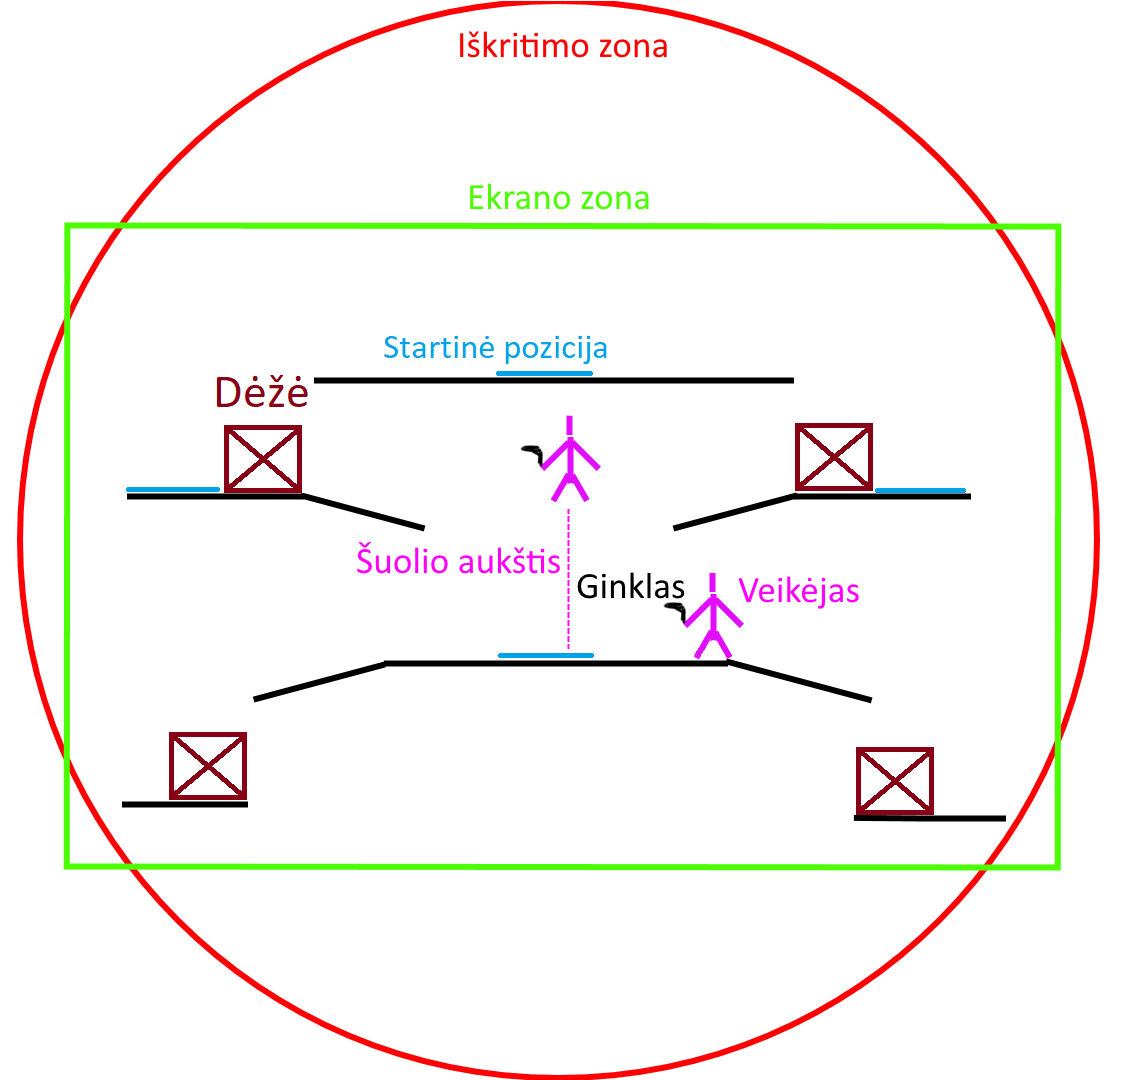
\includegraphics[scale=0.4]{img/Arenas/map1.png}
    \caption{Pirmosios arenos eskizas}
    \label{img:map1}
\end{figure}

\begin{figure}[H]
    \centering
    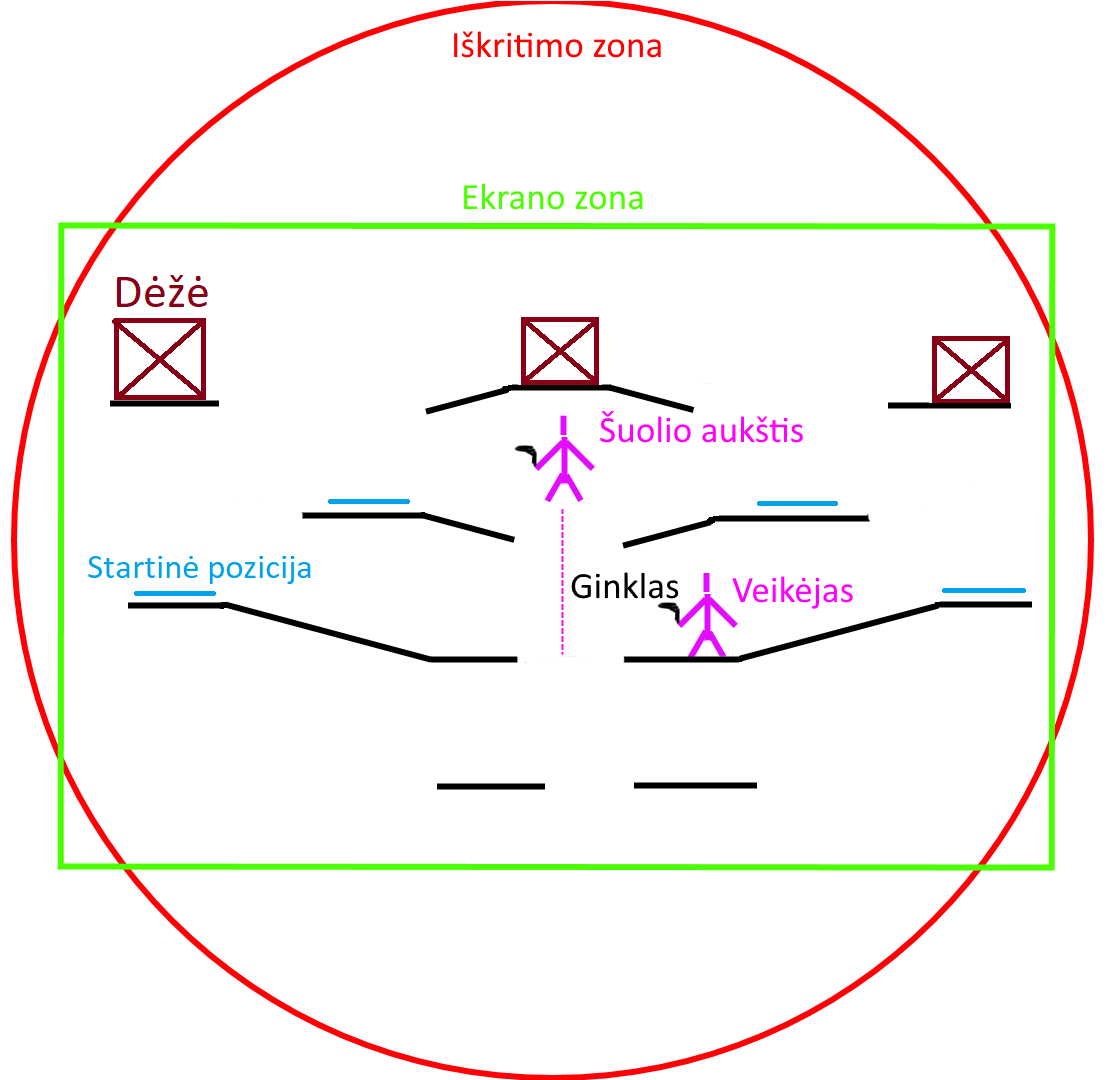
\includegraphics[scale=0.4]{img/Arenas/map2.png}
    \caption{Antrosios arenos eskizas}
    \label{img:map2}
\end{figure}



% -----------------------------------------------------------------
% ----------------------- 3. INTERFEISAS --------------------------
% -----------------------------------------------------------------
\section{Interfeisas}
Tolimesniuose poskyriuose aprašomos žaidimo interfeiso detalės.


% -------------------------------------------
% --------- 3.1 Pagrindinis meniu -----------
% -------------------------------------------
\subsection{Pagrindinis meniu}
Pagrindinio meniu (žr. \ref{img:Main_menu} pav.) fonas yra vaizdo įrašas su žaidimo eiga. Įrašui pasibaigus jis prasideda iš naujo.  Pagrindinio meniu pasirinkimai rodomi apatiniame kairiajame kampe.\newline

Galimi pasirinkimai:
\begin{itemize}
    \item Start game (\textit{Pradėti žaidimą})
    \begin{itemize}
        \item Character selection screen (\textit{Veikėjų pasirinkimo langas}) (žr. \ref{img:Character_choice_menu} pav.)
        \begin{itemize}
            \item Arena selection screen (\textit{Arenos pasirinkimo langas})
        \end{itemize}
    \end{itemize}
    \item Controls (\textit{Valdymas})
    \begin{itemize}
        \item Key bindings screen (\textit{Mygtukų konfigūracijos langas})
    \end{itemize}
    \item Settings (\textit{Nustatymai}) (žr. \ref{img:Settings_menu} pav.)
    \begin{itemize}
        \item Brightness (\textit{Šviesumas})
        \item Resolution (\textit{Žaidimo rezoliucija})
        \item Master volume (\textit{Bendras žaidimo garsumas})
        \item Music volume (\textit{Muzikos garsumas})
        \item Sound effects volume (\textit{Efektų garsumas})
    \end{itemize}
    \item Quit (\textit{Išeiti iš žaidimo})
    \begin{itemize}
        \item Yes (\textit{Taip})
        \item No (\textit{Ne})
    \end{itemize}
\end{itemize}

\begin{figure}[H]
    \centering
    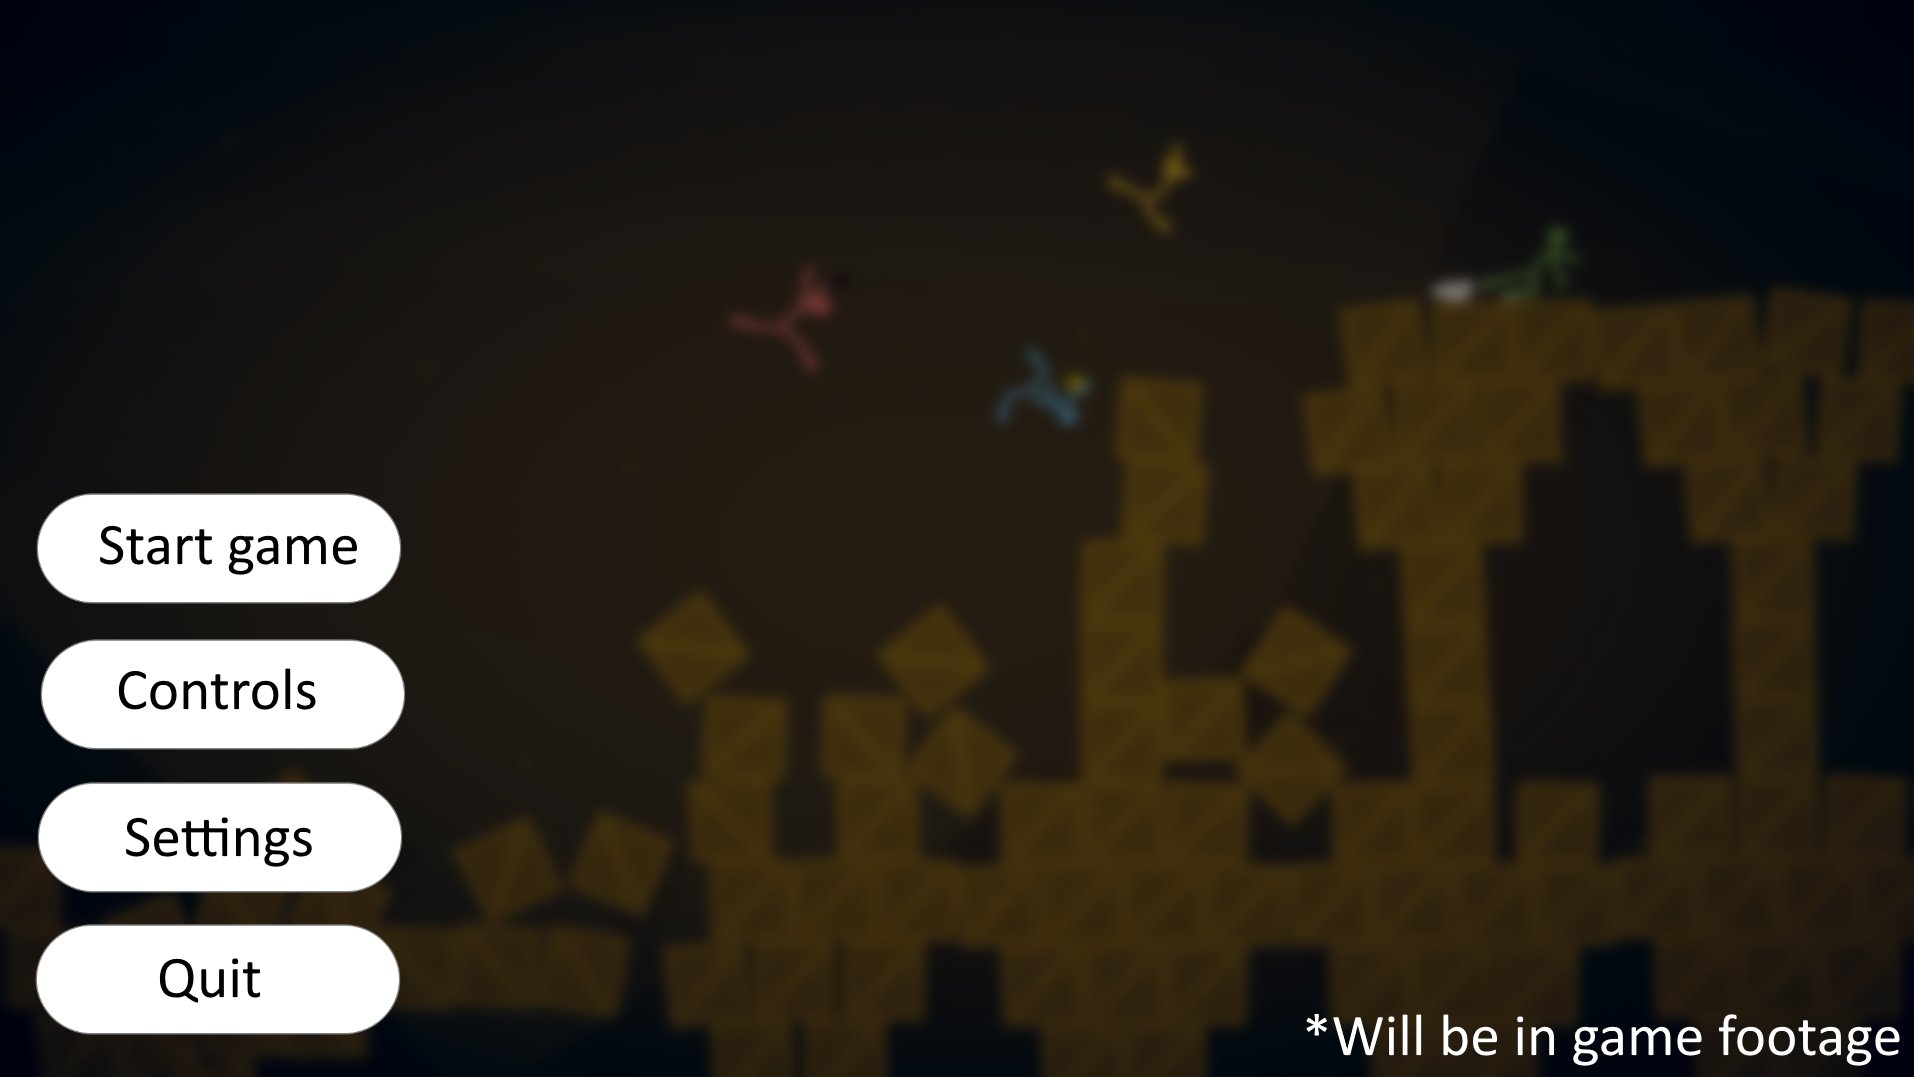
\includegraphics[scale=0.3]{img/Menus/Main.png}
    \caption{Pagrindinio meniu eskizas}
    \label{img:Main_menu}
\end{figure}

\begin{figure}[H]
    \centering
    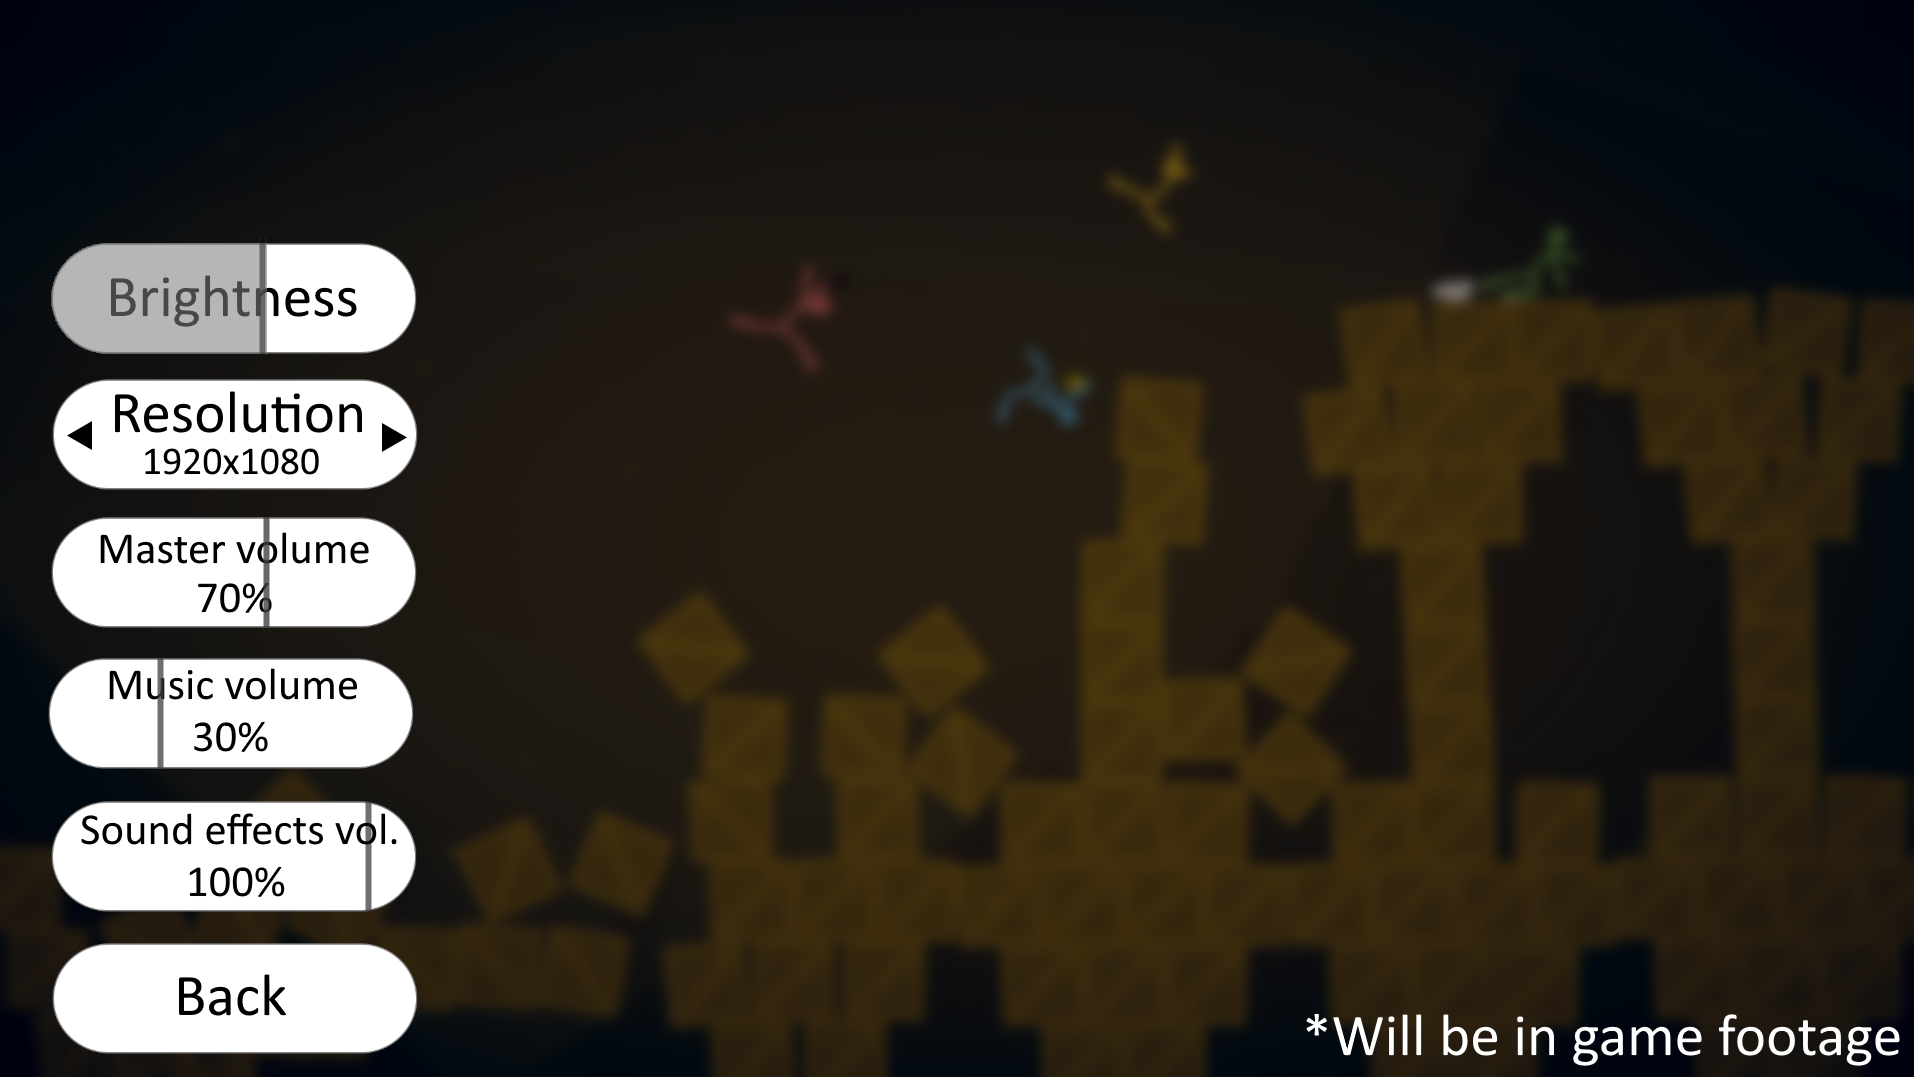
\includegraphics[scale=0.3]{img/Menus/Settings.png}
    \caption{Nustatymų meniu eskizas}
    \label{img:Settings_menu}
\end{figure}

\begin{figure}[H]
    \centering
    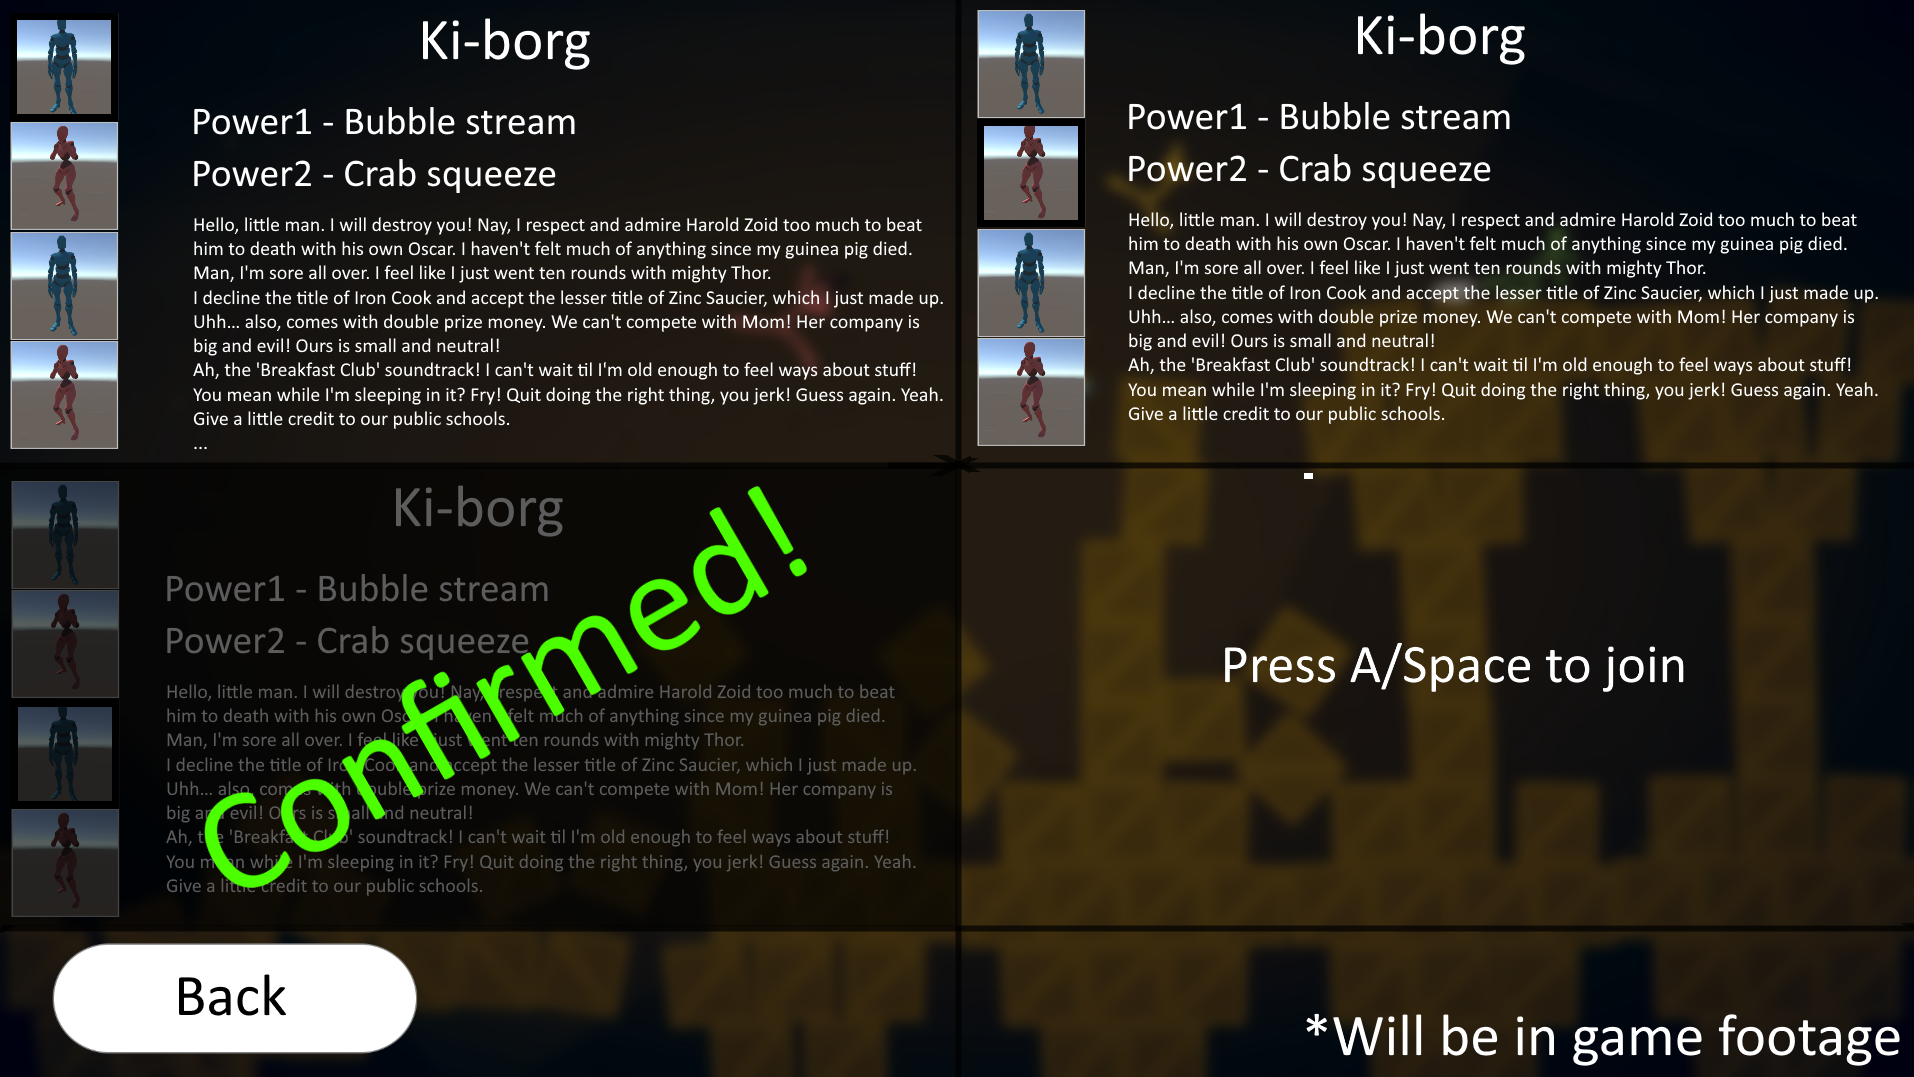
\includegraphics[scale=0.3]{img/Menus/Character_choice.png}
    \caption{Veikėjų pasirinkimo meniu eskizas}
    \label{img:Character_choice_menu}
\end{figure}

% -------------------------------------------
% ------ 3.2 Sustabdyto žaidimo meniu -------
% -------------------------------------------
\subsection{Sustabdyto žaidimo meniu}
Žaidėjui paspaudus meniu mygtuką žaidimas yra sustabdomas, vaizdas patamsinamas bei suliejamas ir ekrano centre parodomi sustabdyto žaidimo meniu pasirinkimai.\newline

Galimi pasirinkimai:
\begin{itemize}
    \item Resume game (\textit{Pratęsti žaidimą});
    \item Settings (\textit{Nustatymai});
    \item Controls (\textit{Valdymas});
    \item Quit (\textit{Grįžti į pagrindinį meniu}).
\end{itemize}


% -------------------------------------------
% ----- 3.3 Veikėjų pasirinkimų langas ------
% -------------------------------------------
\subsection{Veikėjų pasirinkimų langas}
Rodomas užrašas "Press A/Space to join" ir kiekvienam žaidėjui paspaudus atitinkamą mygtuką aktyvuojasi lango sekcija, kuria žaidėjas renkasi veikėją. Tą patį veikėją gali rinktis keli žaidėjai. Visiems žaidėjams patvirtinus savo pasirinkimus atidaromas arenos pasirinkimo langas.

\subsection{Arenos pasirinkimo langas}
Rodomas arenos sumažintas paveiksliukas, arenos pavadinimas ir raundų skaičius. Areną ir raundų skaičių pasirenka pirmas žaidėjas. Patvirtinus pasirinkimus žaidimas pradedamas.


% -------------------------------------------
% ---- 3.4 Mygtukų konfigūracijos langas ----
% -------------------------------------------
\subsection{Mygtukų konfigūracijos reikšmės}
Toliau pateikta lentelė su galimais valdymo pulto bei   klaviatūros ir pelės kombinacijos valdymo mygtukais/klavišais ir juos atitinkančiomis funkcijomis (žr. \ref{tab:BtnConfigs} pav.).


\begin{figure}[h!]
\centering
\caption{Numatytos mygtukų konfigūracijos}
\csvautotabular{Tables/controlDescriptions.csv}
\label{tab:BtnConfigs}
\end{figure}



% -----------------------------------------------------------------
% ----------------------- 4. GARSO STILIUS ------------------------
% -----------------------------------------------------------------
\section{Garso stilius}
Tolimesniuose poskyriuose pateikiami grafikos ir garsų sąrašai


% -------------------------------------------
% ------------ 4.1 Garsų sąrašas ------------
% -------------------------------------------
\subsection{Garsų sąrašas}


% -------------------------------
% -- 4.1.1 Unikalūs veikėjams ---
% -------------------------------
\subsubsection{Unikalūs veikėjams}
Šie garsai yra unikalūs kiekvienam veikėjui:

\begin{itemize}
    \item Veikėjas sužeidžiamas (1 variacija);
    \item Veikėjas sužeidžiamas (2 variacija);
    \item Veikėjas sužeidžiamas (3 variacija);
    \item Veikėjas miršta;
    \item Veikėjo vardo ištarimas (naudojama veikėjo pasirinkimo lange);
    % \item Veikėjo galios pavadinimo ištarimas (naudojama veikėjui panaudojus savo galią).
\end{itemize}

% -------------------------------
% ---- 4.1.2 Bendri veikėjams ---
% -------------------------------
\subsubsection{Bendri veikėjams}
Šie garsai yra bendri visiems žaidimo veikėjams:

\begin{itemize}
    \item Veikėjas smūgiuoja;
    \item Veikėjas pašoka aukštyn (įskaitant dvigubą šuolį);
    \item Veikėjas nusileidžia ant paviršiaus;
    \item Veikėjas dėl varžovo smūgio kyla aukštyn;
    \item Veikėjas miršta, nes per ilgai buvo už apskritimo ribų;
    \item Veikėjas ginasi.
\end{itemize}

% -------------------------------
% -------- 4.1.3 Ginklų ---------
% -------------------------------
\subsubsection{Ginklų}
Ginklams specifiniai garsai:

\begin{itemize}
    \item Pistoleto iššovimas;
    \item Pistoleto atsitrenkimas į paviršių (atsitiktinai atsiradus arenoje);
    \item Automato iššovimas;
    \item Automato atsitrenkimas į paviršių (atsitiktinai atsiradus arenoje);
    \item Šratinio iššovimas;
    \item Šratinio atsitrenkimas į paviršių (atsitiktinai atsiradus arenoje);
    \item Snaiperio iššovimas;
    \item Snaiperio atsitrenkimas į paviršių (atsitiktinai atsiradus arenoje);
    \item Raketsvaidžio iššovimas;
    \item Raketsvaidžio raketos sprogimas;
    \item Raketsvaidžio atsitrenkimas į paviršių (atsitiktinai atsiradus arenoje);
    \item Beisbolo lazdos užsimojimas;
    \item Beisbolo lazdos atsitrenkimas į paviršių (atsitiktinai atsiradus arenoje);
    \item Dalgio užsimojimas;
    \item Dalgio atsitrenkimas į paviršių (atsitiktinai atsiradus arenoje);
    \item Peilio užsimojimas;
    \item Peilio atsitrenkimas į paviršių (atsitiktinai atsiradus arenoje).
\end{itemize}

% -------------------------------
% ---------- 4.1.4 Kiti ---------
% -------------------------------
\subsubsection{Kiti}
Visi kiti žaidime naudojami garsai:

\begin{itemize}
    \item Meniu muzika;
    \item Žaidimo metu grojanti muzika (unikali žemėlapiams);
    \item Veikėjo pasirinkimo patvirtinimas (įskaitant arenos pasirinkimą);
    \item Meniu grįžimas atgal (spaudžiant "Esc");
    \item Meniu pasirinkimo patvirtinimas (spaudžiant "Enter");
    \item Meniu navigavimas (vaikštant pasirinkimais aukštyn/žemyn);
    \item Šviesumo dydžio pasirinkimas;
    \item Pergalių skaičiaus limito pasirinkimas;
    \item Atgalinis skaičiavimas prieš prasidedant kovai.
\end{itemize}



% -----------------------------------------------------------------
% -------------------- 5. DARBŲ TVARKARAŠTIS ----------------------
% -----------------------------------------------------------------
\section{Darbų tvarkaraštis}
Toliau pateikiami patikslinti darbų planas semestro metu (žr. 1 lentelė) ir komandos narių pasiskirstymas darbais (žr. 2 lentelė).

{\centering
\begin{longtable}{|L{3,4cm}|L{8,2cm}|L{1,5cm}|L{1,6cm}|}
\caption{Patikslintas darbų tvarkaraštis}
\label{variability_impl_mech}
\endfirsthead
\endhead
\hline

\textbf{Atlikimo terminas} & 
\textbf{Darbo pavadinimas} & 
\textbf{Apimtis (val.)} & 
\textbf{Žmonių skaičius} \\ \hline

\textbf{Spalio 6 - 13} &
Parašyti projekto ir dizaino dokumentaciją &
10 & 1-2 \\ \hline

\textbf{Spalio 8 - 13} &
Surinkti reikiamą grafiką, garsus, muziką ir paveikslėlius &
2-3 & 1-3 \\ \hline

\textbf{Spalio 14} &
Nusiųsti dokumentaciją dėstytojui &
- & 1 \\ \hline

\textbf{Spalio 15 - 16} &
Pristatyti ir parodyti dokumentaciją, grafikos, audio failus lab. darbų metu &
- & 1-4 \\ \hline

\textbf{Spalio 17 - 30} &
Intensyvus žaidimo vystymo procesas &
18-24 & 3-4 \\ \hline

\textbf{Spalio 29 - lapkričio 2} &
Dokumentacijos atnaujinimas &
3 & 1 \\ \hline

\textbf{
Spalio 31 - lapkričio 3} &
Žaidimo veikimo testavimas.
Žaidimo atitikimo reikalavimams testavimas.
Klaidų taisymas/neįvykdytų reikalavimų integravimas &
2-3 & 2-3 \\ \hline

\textbf{Lapkričio 4} &
Nusiųsti dėstytojui veikiančią pradinę žaidimo versiją ir atnaujintą dokumentaciją &
- & 1 \\ \hline

\textbf{Lapkričio 5 - 6} &
Pradinės žaidimo versijos pristatymas lab. darbų metu &
- & 1-4 \\ \hline

\textbf{Lapkričio 7 - 25} &
Intensyvus žaidimo pilnos versijos kūrimas &
30-40 & 3-4 \\ \hline

\textbf{Lapkričio 26 - gruodžio 1} &
Žaidimo veikimo testavimas.
Žaidimo atitikimo reikalavimams testavimas.
Klaidų taisymas/neįvykdytų reikalavimų integravimas.
Papildomo funkcionalumo pridėjimas &
4-12 & 2-4 \\ \hline

\textbf{Lapkričio 27 - gruodžio 1} &
Paruošti žaidimo pristatomąjį dokumentą &
5 & 1-2 \\ \hline

\textbf{Gruodžio 2} &
Žaidimo pristatomąjį dokumentą nusiųsti dėstytojui &
- & 1 \\ \hline

\textbf{Gruodžio 3 - 4} &
Pristatyti baigtinę žaidimo versiją lab. darbų metu &
- & 1-4 \\ \hline

\textbf{Gruodžio 5 - 7} &
Atlikti konkurentų komandos žaidimo analizę &
4-6 & 2-3 \\ \hline

\textbf{Gruodžio 7 - 8} &
Parengti konkurentų komandos žaidimo apžvelgiamąjį dokumentą &
2-4 & 1 \\ \hline

\textbf{Gruodžio 9} &
Nusiųsti konkurentų komandos žaidimo apžvelgiamąjį dokumentą dėstytojui &
- & 1 \\ \hline

\textbf{Gruodžio 10 - 16} &
Parengti žaidimo eigos vaizdo įrašą, pasiruošti žaidimo pristatymui &
8 & 1-4 \\ \hline

\textbf{Gruodžio 17} &
Pristatyti žaidimą Teorinės paskaitos metu &
- & 1-4 \\ \hline

\end{longtable}}



{\centering
\begin{longtable}{|L{8,6cm}|L{6,1cm}|}
\caption{komandos narių pasiskirstymas darbais}
\label{variability_impl_mech}
\endfirsthead
\endhead
\hline

\textbf{Darbo pavadinimas} & 
\textbf{Atsakingas asmuo} \\ \hline

Intensyvus žaidimo vystymo etapas &
Visa komanda \\ \hline

Atnaujinti dokumentaciją &
Gediminas Krasauskas \\ \hline

Testuoti žaidimo veikimą &
Visa komanda \\ \hline

Testuoti žaidimo atitikimą reikalavimams &
Gediminas Krasauskas \\ \hline

Ištaisyti klaidas ir integruoti neįvykdytus reikalavimus &
Visa komanda \\ \hline

Nusiųsti dėstytojui veikiančią pradinę žaidimo versiją ir atnaujintą dokumentaciją &
Benas Bagdanovas \\ \hline

Pristatyti Pradinę žaidimo versiją lab. darbų metu &
Visa komanda \\ \hline

Intensyvus žaidimo pilnos versijos kūrimo etapas &
Visa komanda \\ \hline

Testuoti žaidimo veikimą &
Visa komanda \\ \hline

Testuoti žaidimo atitikimą reikalavimams &
Gediminas Krasauskas \\ \hline

Ištaisyti klaidas ir integruoti neįvykdytus reikalavimus &
Emilijus Stankus, Karolis Užkuraitis, Gediminas Krasauskas \\ \hline

Pridėti papildomą funkcionalumą &
Karolis Užkuraitis, Benas Bagdanovas, Emilijus Stankus \\ \hline

Paruošti žaidimo pristatomąjį dokumentą &
Benas Bagdanovas, Gediminas Krasauskas \\ \hline

Nusiųsti žaidimo pristatomąjį dokumentą dėstytojui &
Benas Bagdanovas \\ \hline

Pristatyti baigtinę žaidimo versiją lab. darbų metu &
Visa komanda \\ \hline

Atlikti konkurentų komandos žaidimo analizę &
Gediminas Krasauskas, Emilijus Stankus \\ \hline

Parengti konkurentų komandos žaidimo apžvelgiamąjį dokumentą &
Gediminas Krasauskas \\ \hline

Nusiųsti konkurentų komandos žaidimo apžvelgiamąjį dokumentą dėstytojui &
Benas Bagdanovas \\ \hline

Parengti žaidimo eigos vaizdo įrašą &
Emilijus Stankus, Benas Bagdanovas \\ \hline

Pasiruošti žaidimo pristatymui &
Visa komanda \\ \hline

Pristatyti žaidimą Teorinės paskaitos metu &
Visa komanda \\ \hline

\end{longtable}}



% -----------------------------------------------------------------
% --------------------- 6. RESURSŲ ŠALTINIAI ----------------------
% -----------------------------------------------------------------
\section{Resursų šaltiniai}
Pateikiami dokumente referuojamų modelių ir garsų šaltiniai.


% -------------------------------------------
% ----------- 6.1 Veikėjų modeliai ----------
% -------------------------------------------
\subsection{Veikėjų modeliai}
Toliau pateikiamas sąrašas su veikėjais ir jų atitinkančių modelių šaltiniais:
\begin{itemize}
    \item \textbf{Malean} - \textit{Y Bot} (aut. \textit{Mixamo}) (https://www.mixamo.com);
    \item \textbf{Valkyrie} - \textit{X Bot} (aut. \textit{Mixamo}) (https://www.mixamo.com);
    \item \textbf{Penkratjevas} - \textit{Vanguard} (aut. T. Choonyung) (https://www.mixamo.com);
    \item \textbf{Bonbon} - \textit{Sci-Fi Soldier} (aut. Yurov Viktor) (https://assetstore.unity.com/packages/3d/ characters/humanoids/sci-fi-soldier-29559).
\end{itemize}


% -------------------------------------------
% ----------- 6.2 Ginklų modeliai -----------
% -------------------------------------------
\subsection{Ginklų modeliai}
Toliau pateikiamas sąrašas su ginklais ir jų atitinkančių modelių šaltiniais:
\begin{itemize}
    \item \textbf{Pistoletas} - \textit{Low Poly Gun Pack} (aut. DUANE'S MIND) iš \textit{Unity Asset Store} (https://assetstore.unity.com/packages/3d/props/guns/low-poly-gun-pack-4725);
    \item \textbf{Automatas} - \textit{Low Poly Gun Pack} (aut. DUANE'S MIND) iš \textit{Unity Asset Store} (https://assetstore.unity.com/packages/3d/props/guns/low-poly-gun-pack-4725);
    \item \textbf{Šratinis} - \textit{Low Poly Gun Pack} (aut. DUANE'S MIND) iš \textit{Unity Asset Store} (https://assetstore.unity.com/packages/3d/props/guns/low-poly-gun-pack-4725);
    \item \textbf{Snaiperis} - \textit{Low Poly Gun Pack} (aut. DUANE'S MIND) iš \textit{Unity Asset Store} (https://assetstore.unity.com/packages/3d/props/guns/low-poly-gun-pack-4725);
    \item \textbf{Raketsvaidis} - \textit{Low Poly Gun Pack} (aut. DUANE'S MIND) iš \textit{Unity Asset Store} (https://assetstore.unity.com/packages/3d/props/guns/low-poly-gun-pack-4725);
    \item \textbf{Beisbolo lazda} - \textit{Baseball Bats - Pack} (aut. CGUNWALE) iš  \textit{Unity Asset Store} (https://assetstore.unity.com/packages/3d/props/weapons/baseball-bats-pack-102171);
    \item \textbf{Dalgis} - \textit{Skull Scythe} (aut. CALAVERA GAME STUDIO) iš  \textit{Unity Asset Store} (https://assetstore.unity.com/packages/3d/props/weapons/skull-scythe-11982);
    \item \textbf{Peilis} - \textit{M9 Knife} (aut. URBANITY) iš  \textit{Unity Asset Store} (https://assetstore.unity.com/packages/3d/props/weapons/m9-knife-7597).
\end{itemize}


% -------------------------------------------
% --------------- 6.3 Garsai ----------------
% -------------------------------------------
\subsection{Garsai}
Šiame skyriuje pateikiami sąrašai su audio garsais ir jų šaltiniais.


% ---------------------------------------
% ------- 6.3.1 Bendri veikėjams --------
% ---------------------------------------
\subsubsection{Bendri veikėjams}
Toliau pateikiamas sąrašas su bendrais veikėjų audio garsais ir jų šaltiniais:
\item - \textbf{Veikėjas pašoka aukštyn} - \textit{Jump Sound Effects All Sounds} (aut. \textit{All Sounds}) iš (https://www.youtube.com/watch?v=\_eqKyzxa0dM);
\item - \textbf{Veikėjas nusileidžia ant paviršiaus} - \textit{Footstep Free sound effect} (aut. \textit{Free SoundEffects}) iš (https://www.youtube.com/watch?v=B6Ajq-3ivvY);
\item - \textbf{Veikėjas dėl varžovo smūgio kyla aukštyn} - \textit{Swoosh sound effect} (aut. \textit{John Lubiz}) iš (https://www.youtube.com/watch?v=VS9fDfmlJPM);
\item - \textbf{Veikėjas miršta, nes per ilgai buvo už apskritimo ribų} - \textit{Whip Sound Effect} (aut. \textit{Sound Effects}) iš (https://www.youtube.com/watch?v=CQWAtviZ1I4);
\item - \textbf{Veikėjas ginasi} - \textit{Swish, Swoosh, Cutscene Sound Effect} (aut. \textit{Animal Jam Giveaway}) iš (https://www.youtube.com/watch?v=EFY9TX2Fghg).


% ---------------------------------------
% ------ 6.3.2 Unikalūs veikėjams -------
% ---------------------------------------
\subsubsection{Unikalūs veikėjams}
Toliau pateikiamas sąrašas su bendrais veikėjų audio garsais ir jų šaltiniais:

\item - \textbf{Malean veikėjas sužeidžiamas (1 variacija)} (aut. \textit{Emilijus Stankus});
\item - \textbf{Malean veikėjas sužeidžiamas (2 variacija)} (aut. \textit{Emilijus Stankus});
\item - \textbf{Malean veikėjas sužeidžiamas (3 variacija)} (aut. \textit{Emilijus Stankus});
\item - \textbf{Malean veikėjas miršta} (aut. \textit{Emilijus Stankus});
\item - \textbf{Malean veikėjo vardo ištarimas} (aut. \textit{Emilijus Stankus});

\item - \textbf{Valkyrie veikėjas sužeidžiamas (1 variacija)} (aut. \textit{Benas Bagdanovas});
\item - \textbf{Valkyrie veikėjas sužeidžiamas (2 variacija)} (aut. \textit{Benas Bagdanovas});
\item - \textbf{Valkyrie veikėjas sužeidžiamas (3 variacija)} (aut. \textit{Benas Bagdanovas});
\item - \textbf{Valkyrie veikėjas miršta} (aut. \textit{Benas Bagdanovas});
\item - \textbf{Valkyrie veikėjo vardo ištarimas} (aut. \textit{Benas Bagdanovas});

\item - \textbf{Penkratjev veikėjas sužeidžiamas (1 variacija)} (aut. \textit{Gediminas Krasauskas});
\item - \textbf{Penkratjev veikėjas sužeidžiamas (2 variacija)} (aut. \textit{Gediminas Krasauskas});
\item - \textbf{Penkratjev veikėjas sužeidžiamas (3 variacija)} (aut. \textit{Gediminas Krasauskas});
\item - \textbf{Penkratjev veikėjas miršta} (aut. \textit{Gediminas Krasauskas});
\item - \textbf{Penkratjev veikėjo vardo ištarimas} (aut. \textit{Gediminas Krasauskas});

\item - \textbf{Bonbon veikėjas sužeidžiamas (1 variacija)} (aut. \textit{Karolis Užkuraitis});
\item - \textbf{Bonbon veikėjas sužeidžiamas (2 variacija)} (aut. \textit{Karolis Užkuraitis});
\item - \textbf{Bonbon veikėjas sužeidžiamas (3 variacija)} (aut. \textit{Karolis Užkuraitis});
\item - \textbf{Bonbon veikėjas miršta} (aut. \textit{Karolis Užkuraitis});
\item - \textbf{Bonbon veikėjo vardo ištarimas} (aut. \textit{Karolis Užkuraitis}).


% -------------------------------
% ------- 6.3.3 Ginklai ---------
% -------------------------------
\subsubsection{Ginklai}
Toliau pateikiamas sąrašas su ginklų audio garsais ir jų šaltiniais:
\begin{itemize}
    % Pistoletas
    \item \textbf{Pistoleto iššovimas} - \textit{All the old CS:GO Sounds} (aut. \textit{Josh McKendry}) iš (https://www.youtube.com/watch?v=pVlVBVlkuus);
    \item \textbf{Pistoleto atsitrenkimas į paviršių (atsitiktinai atsiradus arenoje)} - \textit{Gun Drop on Cement [SOUND EFFECT]} (aut. \textit{Freeify Music}) iš (https://www.youtube.com/watch?v=5vfcYDgvQsk);
    % Automatas
    \item \textbf{Automato iššovimas} - \textit{All the old CS:GO Sounds} (aut. \textit{Josh McKendry}) iš (https://www.youtube.com/watch?v=pVlVBVlkuus);
    \item \textbf{Automato atsitrenkimas į paviršių (atsitiktinai atsiradus arenoje)} - \textit{Gun Drop on Cement [SOUND EFFECT]} (aut. \textit{Freeify Music}) iš (https://www.youtube.com/watch?v=5vfcYDgvQsk);
    % Šratinis
    \item \textbf{Šratinio iššovimas} - \textit{All the old CS:GO Sounds} (aut. \textit{Josh McKendry}) iš (https://www.youtube.com/watch?v=pVlVBVlkuus);
    \item \textbf{Šratinio atsitrenkimas į paviršių (atsitiktinai atsiradus arenoje)} - \textit{Gun Drop on Cement [SOUND EFFECT]} (aut. \textit{Freeify Music}) iš (https://www.youtube.com/watch?v=5vfcYDgvQsk);
    % Snaiperis
    \item \textbf{Snaiperio iššovimas} - \textit{All the old CS:GO Sounds} (aut. \textit{Josh McKendry}) iš (https://www.youtube.com/watch?v=pVlVBVlkuus);
    \item \textbf{Snaiperio atsitrenkimas į paviršių (atsitiktinai atsiradus arenoje)} - \textit{Gun Drop on Cement [SOUND EFFECT]} (aut. \textit{Freeify Music}) iš (https://www.youtube.com/watch?v=5vfcYDgvQsk);
    % Raketsvaidis
    \item \textbf{Raketsvaidžio iššovimas} - \textit{Modern Warfare 2 All Weapons + Camos Gameplay} (aut. \textit{Undeath92}) iš (https://www.youtube.com/watch?v=Nglhgj1Zy3c);
    \item \textbf{Raketsvaidžio raketos sprogimas} - \textit{Explosion and Action Sound Effects} (aut. \textit{Pigment Ajans - Visual Effects}) iš (https://www.youtube.com/watch?v=qfcCNzESwKk);
    \item \textbf{Raketsvaidžio atsitrenkimas į paviršių (atsitiktinai atsiradus arenoje)} - \textit{Gun Drop on Cement [SOUND EFFECT]} (aut. \textit{Freeify Music}) iš (https://www.youtube.com/watch?v=5vfcYDgvQsk);
    % Beisbolas
    \item \textbf{Beisbolo lazdos užsimojimas} - \textit{Swoosh Whoosh Sword Air Swing Sound Effect} (aut. Iwan Sounds and DIY) iš (https://www.youtube.com/watch?v=9eUFdAquFJs);
    \item \textbf{Beisbolo lazdos atsitrenkimas į paviršių (atsitiktinai atsiradus arenoje)} - \textit{Gun Drop on Cement [SOUND EFFECT]} (aut. \textit{Freeify Music}) iš (https://www.youtube.com/watch?v=5vfcYDgvQsk);
    % Dalgis
    \item \textbf{Dalgio užsimojimas} - \textit{Swoosh Whoosh Sword Air Swing Sound Effect} (aut. Iwan Sounds and DIY) iš (https://www.youtube.com/watch?v=9eUFdAquFJs);
    \item \textbf{Dalgio atsitrenkimas į paviršių } - \textit{Gun Drop on Cement [SOUND EFFECT]} (aut. \textit{Freeify Music}) iš (https://www.youtube.com/watch?v=5vfcYDgvQsk);
    % Peilis
    \item \textbf{Peilio užsimojimas} - \textit{Swoosh Whoosh Sword Air Swing Sound Effect} (aut. Iwan Sounds and DIY) iš (https://www.youtube.com/watch?v=9eUFdAquFJs);
    \item \textbf{Peilio atsitrenkimas į paviršių (atsitiktinai atsiradus arenoje)} - \textit{Gun Drop on Cement [SOUND EFFECT]} (aut. \textit{Freeify Music}) iš (https://www.youtube.com/watch?v=5vfcYDgvQsk).
\end{itemize}


% -------------------------------
% --------- 6.3.4 Meniu ---------
% -------------------------------
\subsubsection{Meniu}
Toliau pateikiamas meniu navigavimo garsų sąrašas:
\begin{itemize}
    \item \textbf{Meniu muzika} - \textit{I'll Be There For You} (aut. \textit{The Rembrandts}) iš (https://www.youtube.com/watch?v=2VbODnX0dVs);
    \item \textbf{Meniu navigacijos garsai} - \textbf{UI Sfx} iš (https://assetstore.unity.com/packages/audio/sound-fx/ui-sfx-36989).
\end{itemize}




\end{document}





% ---------------------------------------------
% ------------ NEPANAUDOTOS GALIOS ------------
% ---------------------------------------------

% Enrage - double damage double push from weapons for 4 seconds
% Stone form - no push back for 3 seconds
% Charge - can be canceled any time, if hits then mega pushback, 1 second to start
% Mirror - aktyvavus galią priešininkai pajus savo pačių vaistus
% C4 - panaudojus ten kur stovi padedamas C4 sprogmuo ir su tuo pačiu mygtuku galima detonuoti. C4 laikosi 5 sekundes kol išnyksta
% Vėjų vėjas - priešais esantys priešininkai yra stipriai stumiami 2 sekundes
% Teleportacija - ten kur atsisukęs teleportuojiesi per 10 vienetų
% Garso banga - visi esantys per 10 vienetų atstumą nubloškiami į šonus
% Metimas - bando pagriebti ir jei pagriebia tai meta priešininką
% Slide - slysta priekin pamušdamas stovinčius priešus aukštyn
% Atsigydymas - atsigydai
% Tornadas - tornadina
% Gervė - prisikabini prie veikėjo ir artėji prie jo nesustodamas ir atsitrenki ten į jį tada ir nustumi
% Dyglys - aktyvavus ir atsitrenkus į priešininką jis prikimba prie tavęs trumpam laikui. Pasibaigus laikui jo greitis būna dvigubas taviškiam
% Greituolis - artimiausio priešo padvigubėja greitis ir jis negali sustoti)(atsiranda greičio akiniai
% Smalkių dūmai - paskleidi dūmus ir visi patekę į sūmus gauna tekę į jų zoną gauna žalos
% One punch - veikėjas pakelia žalą kitam iki 999\%, labai mažas atstumas
% Boxing glove - išlenda bokso kumštis kuris smūgiuoja artimiausią priešininką (bet kiaurai sienas neina)
% Neko - Paverčia kitą veikėją į katiną
% Pagiežingas žvilgsnis - priešininkas, esantis toje kryptyje, kur yra atsisukęs galią aktyvavęs žaidėjas, tampa paralyžiuotas, t.y. 2 sekundes negali pajudėti ir atlikti jokių veiksmų.